
\emph{Global} formulae relate several hidden ground atoms. We use them for two 
purposes: to ensure consistency between the decisions of all SRL stages and to 
capture some of our intuition about the task. We will refer to formulae that 
serve the first purpose as \emph{structural constraints}. 

For example, a structural constraint is given by the (deterministic) formula
\[role(p,a,r) \Rightarrow hasRole(p,a)\]
which ensures that, whenever the argument $a$ is given a label $r$ with respect 
to the predicate $p$, this argument must be an argument of $a$ as denoted by 
\emph{hasRole(p,a)}.

The global formulae that capture our intuition about the task itself can be 
further divided into two classes. The first one uses deterministic or 
\emph{hard} constraints such as
\begin{eqnarray*}
 &role\left(p,a_{1},r\right)\wedge \neg mod\left(r\right)\wedge a_{1}\neq a_{2}  \Rightarrow\\
  & \neg role\left(p,a_{2},r\right)
\end{eqnarray*}
which forbids cases where distinct arguments of a predicate have the same role 
unless the role describes a modifier.

The second class of global formulae is \emph{soft} or nondeterministic. For 
instance, the formula
\begin{eqnarray*}
  & lemma(p,+l) \wedge ppos(a,+p)  \\
  & \wedge hasRole(p,a)  \Rightarrow sense(p,+f) 
\end{eqnarray*}
is a soft global formula. It captures the observation that the sense of a verb 
or noun depends on the type of its arguments. Here the type of an argument token 
is represented by its POS tag.

Simirlarly to the local formulae, the model would include global formulae for 
the \emph{sense/2} predicate depending if the corpus for a specific languages 
models the sense of a SRL predicate. More detail information about the 
structural formulae can be found in previous work 
\citep{riedel08conll,meza09jointly}.

\begin{figure}
\begin{center}
   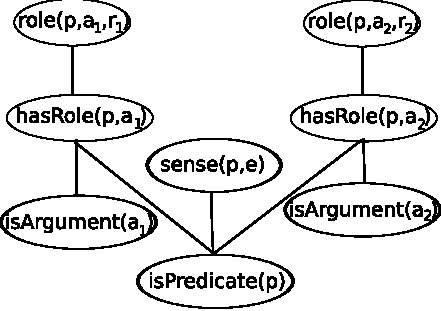
\includegraphics[scale=.70]{GlobalFormula2}
\end{center}
\caption{Markov Network that illustrates the structural constraints we use.}
\label{fig:global2}
\end{figure}




